\documentclass[hyperref={pdfpagelabels=false}]{beamer}
\usepackage{lmodern}


\usetheme{Antibes}




\title{Beamer Class Usetheme Berkeley}  
\author{Sascha Frank} 
\date{\today} 
\begin{document}
%\logo{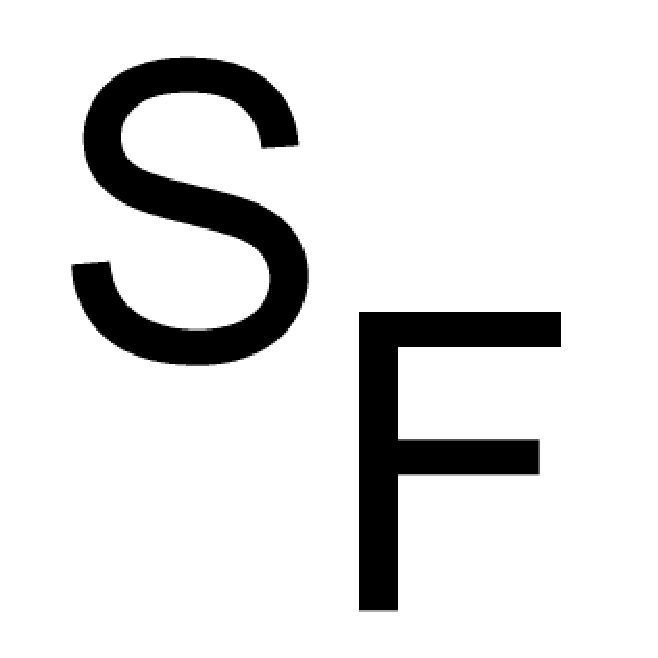
\includegraphics[scale=0.14]{logo-SF}}
\begin{frame}
\titlepage
\end{frame} 


\begin{frame}
\frametitle{Table of contents}
\tableofcontents
\end{frame} 


\section{Section no.1} 
\begin{frame}
\frametitle{frame title} 
Each frame should have a title.
\end{frame}
\subsection{Subsection no.1.1  }
\begin{frame}
Without title somethink is missing. 
\end{frame}


\section{Section no. 2} 
\subsection{Lists I}
\begin{frame}
\frametitle{unnumbered lists}
\begin{itemize}
\item Introduction to  \LaTeX{}  
\item Course 2 
\item Termpapers and presentations with \LaTeX{}  
\item Beamer class
\end{itemize} 
\end{frame}

\begin{frame}\frametitle{lists with single pauses}
\begin{itemize}
\item Introduction to  \LaTeX{}  \pause 
\item Course 2 \pause 
\item Termpapers and presentations with \LaTeX{}  \pause 
\item Beamer class
\end{itemize} 
\end{frame}

\begin{frame}\frametitle{lists with pause}
\begin{itemize}[<+->]
\item Introduction to  \LaTeX{}  
\item Course 2
\item Termpapers and presentations with \LaTeX{}  
\item Beamer class
\end{itemize} 
\end{frame}



\subsection{Lists II}
\begin{frame}\frametitle{numbered lists}
\begin{enumerate}
\item Introduction to  \LaTeX{}   
\item Course 2 
\item Termpapers and presentations with \LaTeX{}  
\item Beamer class
\end{enumerate}
\end{frame}

\begin{frame}
\frametitle{numbered lists with single pauses}
\begin{enumerate}
\item Introduction to  \LaTeX{}  \pause 
\item Course 2 \pause 
\item Termpapers and presentations with \LaTeX{}  \pause 
\item Beamer class
\end{enumerate}
\end{frame}

\begin{frame}
\frametitle{numbered lists with pause}
\begin{enumerate}[<+->]
\item Introduction to  \LaTeX{}  
\item Course 2
\item Termpapers and presentations with \LaTeX{}  
\item Beamer class
\end{enumerate}
\end{frame}




\section{Section no.3} 
\subsection{Tables}
\begin{frame}
\frametitle{Tables}
\begin{tabular}{|c|c|c|}
\hline
\textbf{Date} & \textbf{Instructor} & \textbf{Title} \\
\hline
WS 04/05 & Sascha Frank & First steps with  \LaTeX  \\
\hline
SS 05 & Sascha Frank & \LaTeX \ Course serial \\
\hline
\end{tabular}
\end{frame}


\begin{frame}
\frametitle{Tables with pause}
\begin{tabular}{c c c}
A & B & C \\ 
\pause 
1 & 2 & 3 \\  
\pause 
A & B & C \\ 
\end{tabular} 
\end{frame}


\section{Section no. 4}
\subsection{blocs}
\begin{frame}
\frametitle{blocs}

\begin{block}{title of the bloc}
bloc text
\end{block}

\begin{exampleblock}{title of the bloc}
bloc text
\end{exampleblock}


\begin{alertblock}{title of the bloc}
bloc text
\end{alertblock}
\end{frame}

\end{document}

